% ----------------------------------------------------------------------------------
% ----------------------------------------------------------------------------------

\chapter{Respuesta en frecuencia}

\begin{Resumen}

En este capítulo se describe el método de la respuesta en frecuencia para el análisis y diseño de sistemas de control continuos lineales e invariantes en el tiempo. En la \autoref{sec:frec:intro} se realiza una introducción al análisis en frecuencia. En la \autoref{sec:frec:Fourier} se describe la transformada de Fourier, y en la  \autoref{sec:frec:RespArmonicas} se analiza la respuesta temporal en régimen permanente de un sistema continuo lineal ante una señal armónica.

\end{Resumen}

% ----------------------------------------------------------------------------------
\section{Introducción}
\label{sec:frec:intro}

El tema que aquí se desarrolla corresponde a la asignatura \textsl{Comportamiento Dinámico de
Sistemas} \parencite{sala00,Blasco01}.

El presente tema, \lq\lq Respuesta en frecuencia\rq\rq, es el último propuesto para la
asignatura en cuestión, y se sitúa tras el de \lq\lq Análisis de sistemas dinámicos\rq\rq, en
el que se presentan los conceptos de:

\begin{itemize}

	\item Concepto de estabilidad BIBO. Criterios de estabilidad para sistemas discretos y
	continuos. Estabilidad relativa.
	
	\item Sistemas continuos de primer orden: constante de tiempo, ganancia, respuesta impulsional,
	respuesta ante escalón (tiempo de establecimiento) y respuesta ante rampa.

	\item Sistemas continuos de segundo orden: frecuencia natural y propia, factor de
	decrecimiento, coeficiente de amortiguamiento, respuesta impulsional, respuesta ante escalón
	(sobreoscilación, tiempo de establecimiento, tiempo de pico, etc.) y respuesta ante rampa.

	\item Reducción de sistemas de orden superior: polos dominantes.

	\item Respuesta ante entradas de duración corta: aproximación por la respuesta impulsional.

\end{itemize}

todos ellos basados en el empleo de la función de transferencia y/o del modelo
dinámico de los sistemas bajo estudio.

Consecuentemente, los alumnos ya están familiarizados con la mayoría de las herramientas
básicas para el análisis de sistemas continuos y discretos. Sin embargo, aún no se ha tratado
ningún aspecto relativo al análisis en frecuencia. Por ello, en este último tema se pretende
que los alumnos adquieran las ideas básicas sobre esta herramienta de análisis, relativas sólo
al caso de sistemas continuos.

\begin{parrafoDestacado}

La respuesta en frecuencia para sistemas continuos estudia el comportamiento de los
mismos en régimen permanente cuando se les aplican señales de entrada periódicas, y en
particular armónicas o senoidales, de frecuencia variable desde cero a infinito.

\end{parrafoDestacado}

Una de las razones que justifica el estudio de la respuesta en frecuencia de sistemas continuos
son las diferentes aplicaciones que la ingeniería hace de ella:

\begin{itemize}

	\item \textsl{Telecomunicaciones}. La televisión y la radio se transmiten por el espacio mediante
	ondas electromagnéticas portadoras de frecuencia muy elevada, las cuales excitan a las antenas
	permitiendo su recepción.
	
	\item \textsl{Electrónica}. En las aplicaciones analógicas de la electrónica, tanto de potencia como
	de pequeña señal, es necesario conocer el comportamiento de los circuitos ante señales periódicas
	pertenecientes a un determinado rango de frecuencias. Aplicaciones típicas son los amplificadores de
	sonido y la transmisión de señales por las líneas telefónicas.
	
	\item \textsl{Sistemas eléctricos}. En las redes eléctricas domésticas e industriales tensión de la
	red varía de forma senoidal. En la mayoría de análisis de dichos sistemas se realiza la suposición de
	que el sistema ha llegado al régimen permanente ante la tensión de red senoidal, sin importar el
	régimen transitorio, pues suele ser de muy corta duración.
	
	\item \textsl{Sistemas mecánicos}. El estudio de las vibraciones en los sistemas mecánicos se basa en
	el análisis de los mismos en régimen permanente ante entradas periódicas dentro de un determinado
	rango de frecuencias. Por ejemplo, se analiza la influencia de las vibraciones ocasionadas por el
	viento sobre los edificios, se estudia el efecto de las vibraciones de una determinada máquina de
	fabricación industrial para el diseño de la bancada sobre la que ha de colocarse, con la finalidad de
	amortiguar la propagación de mismas.
	
	\item \textsl{Sistemas  térmicos}. En los estudios sobre calefacción y refrigeración se emplea la
	hipótesis de que la temperatura exterior varia de forma senoidal a lo largo de un día, de esta forma
	se consigue simplificar el estudio y se obtienen soluciones bastante aproximadas.

\end{itemize}


Además de su aplicabilidad a diferentes ramas de la ingeniería, el análisis en frecuencia es
útil en el área de conocimiento de \textsl{Ingeniería de Sistemas y Automática}, entre otros
aspectos, para el diseño de reguladores o compensadores en frecuencia, que presenten
especificaciones típicas del análisis en frecuencia: ancho de banda, frecuencia de resonancia,
atenuación, etc.

% ----------------------------------------------------------------------------------
\section{Señales periódicas. Transformada de Fourier}
\label{sec:frec:Fourier}

Dado que las señales periódicas, y en particular las senoidales, son la base el análisis en
frecuencia, en esta sección se presentan sus propiedades más importantes.

Las señales periódicas son aquellas que satisfacen la condición:

\begin{equation*}
	g(t) = g(t+T) \quad \forall t
\end{equation*}

donde a $T$ se le denomia periodo de la señal y a su inversa frecuencia $f=1/T$. Al
producto de la frecuencia por $2\pi$ se le denomina pulsación de la señal $\omega =2\pi f$. En
el S.I. la unidad de la frecuencia es el $\mathrm{Hz}$ mientras que la de la pulsación es el 
$\si[per-mode=symbol]{\radian\per\second}$, aunque las dos magnitudes tienen la misma dimensión. Normalmente en 
ingeniería, a la pulsación se la suele denominar también frecuencia, de ahí que en el resto del 
tema se la referencie así.


Dentro de las señales periódicas las más importantes son las señales armónicas:

\ifEBOOKPDF
\begin{gather*}
	A\cos(\omega t+\phi), \quad A\sen (\omega t+\phi), \\  A\on{e}^{j\omega t + \phi} = 
		A\cos (\omega t + \phi) + jA\sen (\omega t + \phi) \\[1ex] 
	A\cos (\omega t + \phi) = 
		A\frac{\on{e}^{j(\omega t + \phi) } + \on{e}^{-j(\omega t + \phi)}}{2}\\[1ex]
	A\sen (\omega t + \phi ) = 
		A\frac{\on{e}^{j(\omega t + \phi )}-\on{e}^{-j(\omega t + \phi )}}{2j}
\end{gather*}
\else
\begin{gather*}
	A\cos(\omega t+\phi), \quad A\sen (\omega t+\phi), \quad  A\on{e}^{j\omega t + \phi} = 
		A\cos (\omega t + \phi) + jA\sen (\omega t + \phi) \\[1ex] 
	A\cos (\omega t + \phi) = 
		A\frac{\on{e}^{j(\omega t + \phi) } + \on{e}^{-j(\omega t + \phi)}}{2}\\[1ex]
	A\sen (\omega t + \phi ) = 
		A\frac{\on{e}^{j(\omega t + \phi )}-\on{e}^{-j(\omega t + \phi )}}{2j}
\end{gather*}
\fi

La razón que justifica esta importancia es la posibilidad de descomponer cualquier señal periódica
como una suma de señales armónicas de frecuencia múltiplo de la suya. Esta afirmación se basa en el
\textbf{desarrollo en serie de Fourier}, puesto que dada una señal periódica $g(t)$ de periodo $T$
ésta puede ser descompuesta como sigue:

\begin{equation*}
	g(t) = \sum_{k=-\infty }^{k=\infty }g_{k}\on{e}^{jk\omega t} 
\end{equation*}

siendo los coeficientes de la descomposición:

\begin{equation}
	g_{k} = \dfrac{1}{T}\int _{t_0}^{t_0+T} g(\tau)\on{e}^{-jk\omega \tau } d\tau
		\quad \forall \ t_0 \label{SerieFourier}
\end{equation}

El conjunto de todos los coeficientes $g_{k}$ reciben el nombre de espectro en frecuencia de la señal
periódica en cuestión.

% -------------------------------------------------
% -------------------------------------------------

\begin{ejemplo}

La señal cuadrada que se muestra en la \autoref{cuadrada} es periódica de periodo 1 s. Su
descomposición en serie de Fourier es:

\[
	g_k = \int_0^1 g(\tau)\on{e}^{-jk\cdot 2\pi\cdot \tau} d\tau = 
	\left\{
	\begin{array}{cl}
		 0 & k \text{ par}\\
		\dfrac{2}{k\pi j} & k \text{ impar} 
	\end{array}
	\right.
\]

\ifEPUB
	% No incluimos aquí la figura si es EPUB
\else
	\begin{figure}[htbp]\centering
		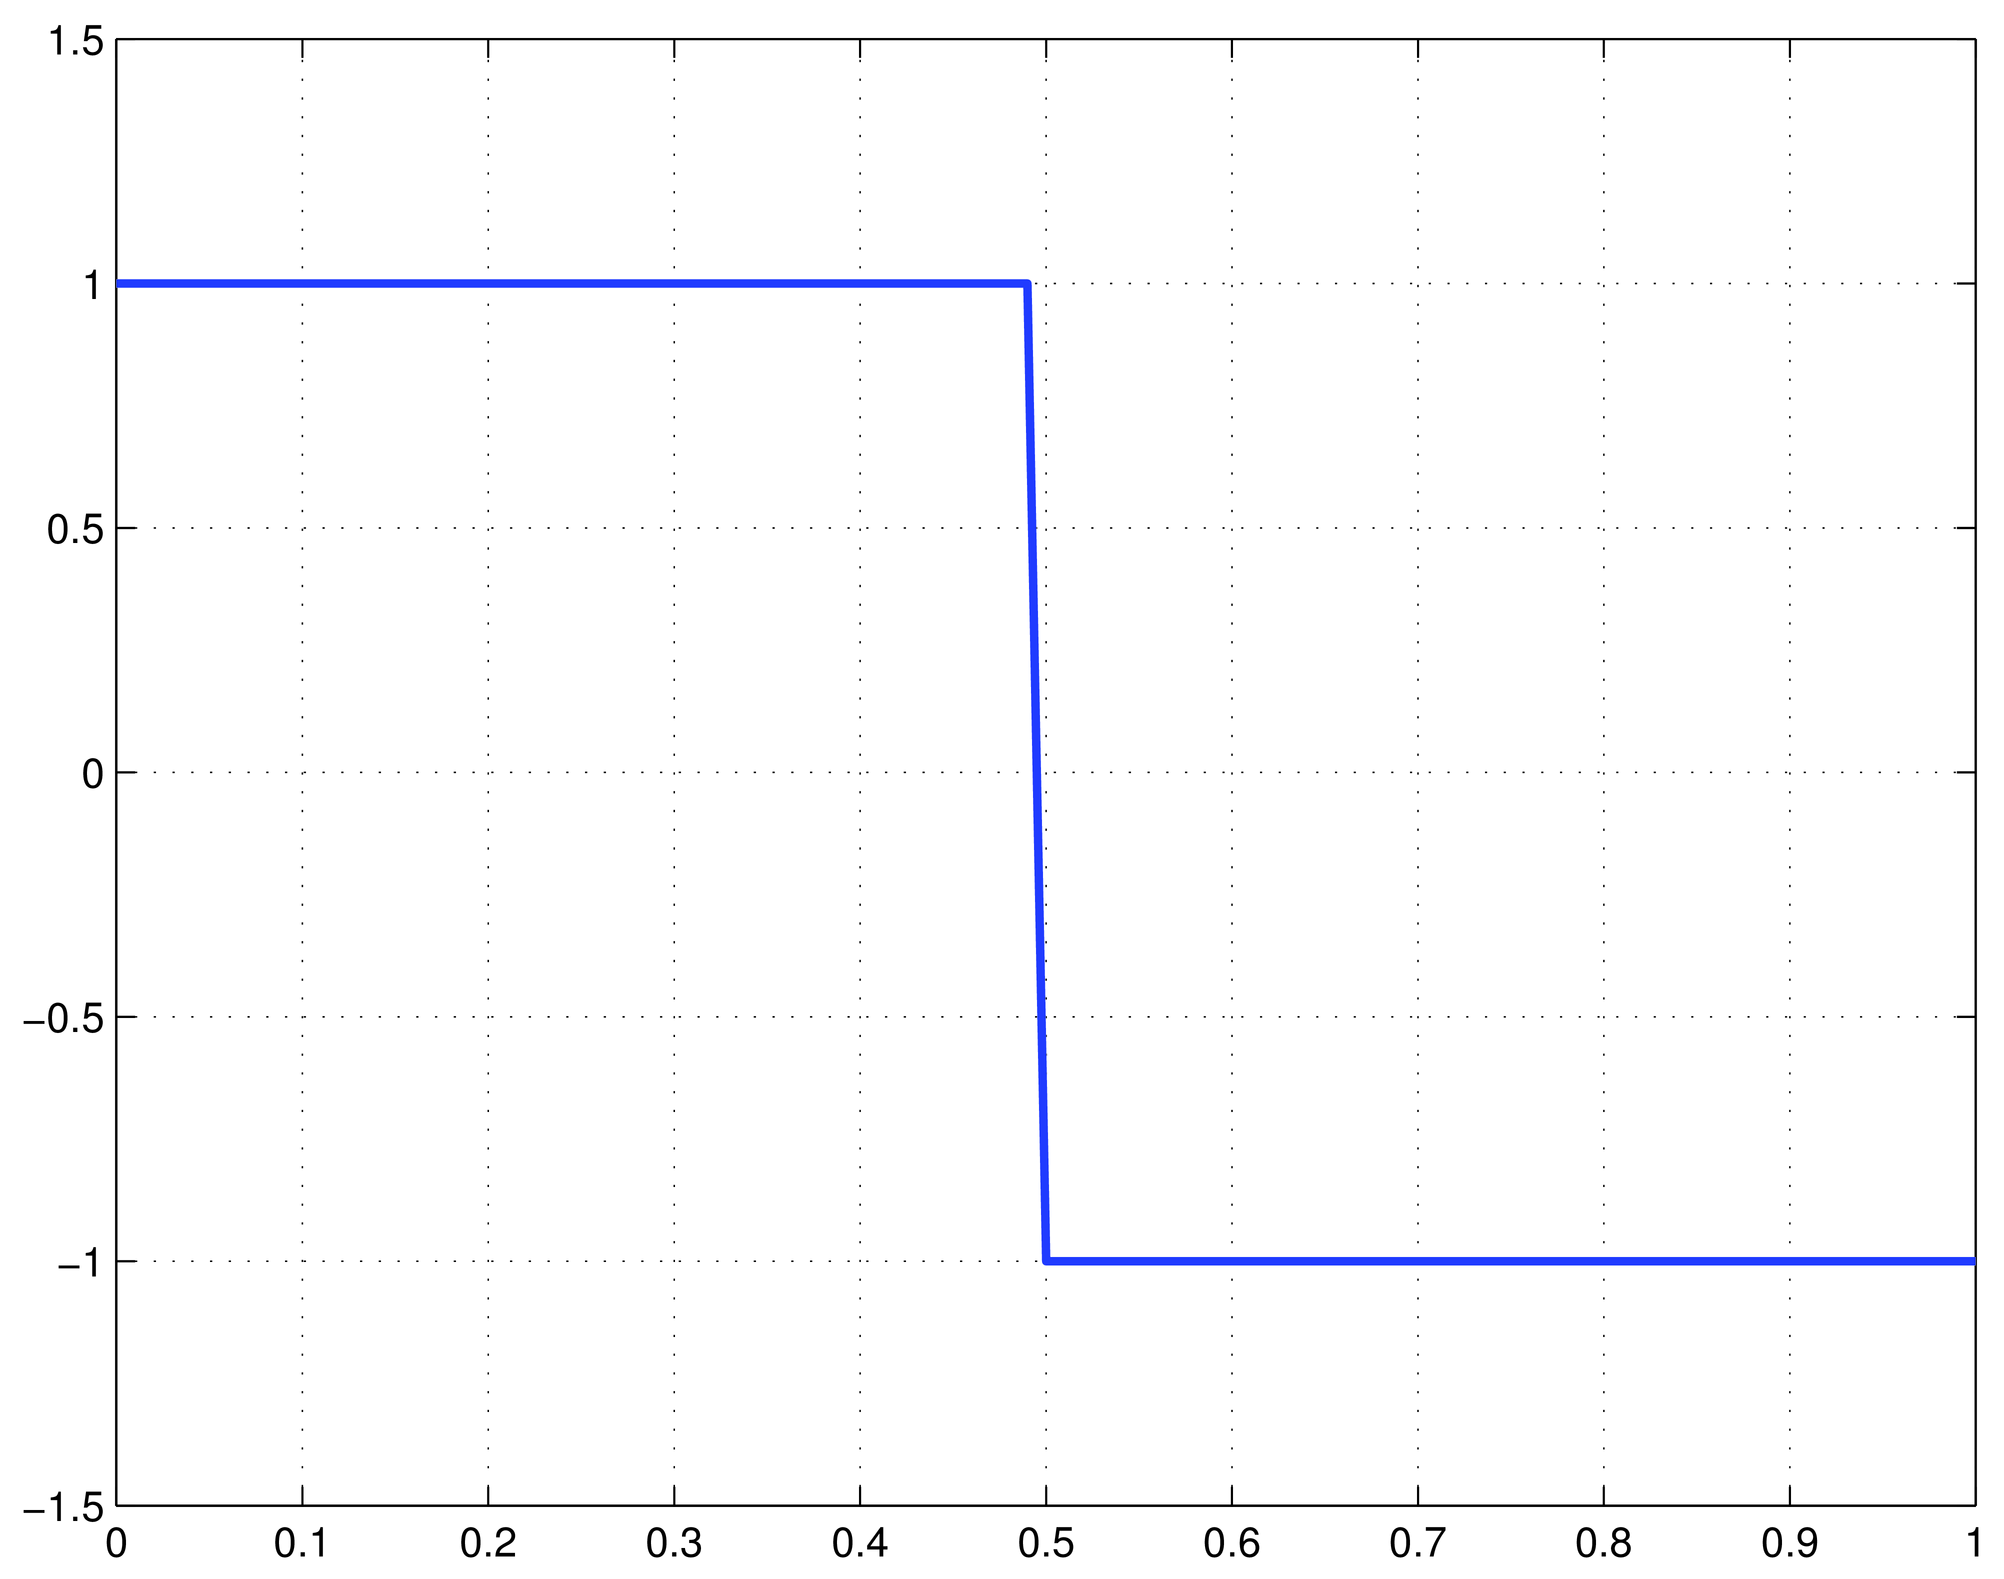
\includegraphics[width=.65\textwidth]{cuadrada}
		\caption{Señal cuadrada de periodo 1 s}
		\label{cuadrada}
		\bigskip
	\end{figure}
\fi

En la \autoref{fig:fourier} se muestran varias aproximaciones de la señal cuadrada mediante
sumas truncadas del desarrollo de Fourier. En particular se han trazado las correspondientes a
truncar hasta $k=$ 1, 3 y 5.

En la \autoref{fig:espectro} se muestra el módulo de los factores $g_k$ correspondientes a diferentes
valores de $k$, constituyendo el denominado espectro de la señal cuadrada.

\end{ejemplo}

% -------------------------------------------------
% -------------------------------------------------


\ifEPUB % Sacamos la figura fuera del ejemplo si es EPUB
	\begin{figure}[htbp]\centering
		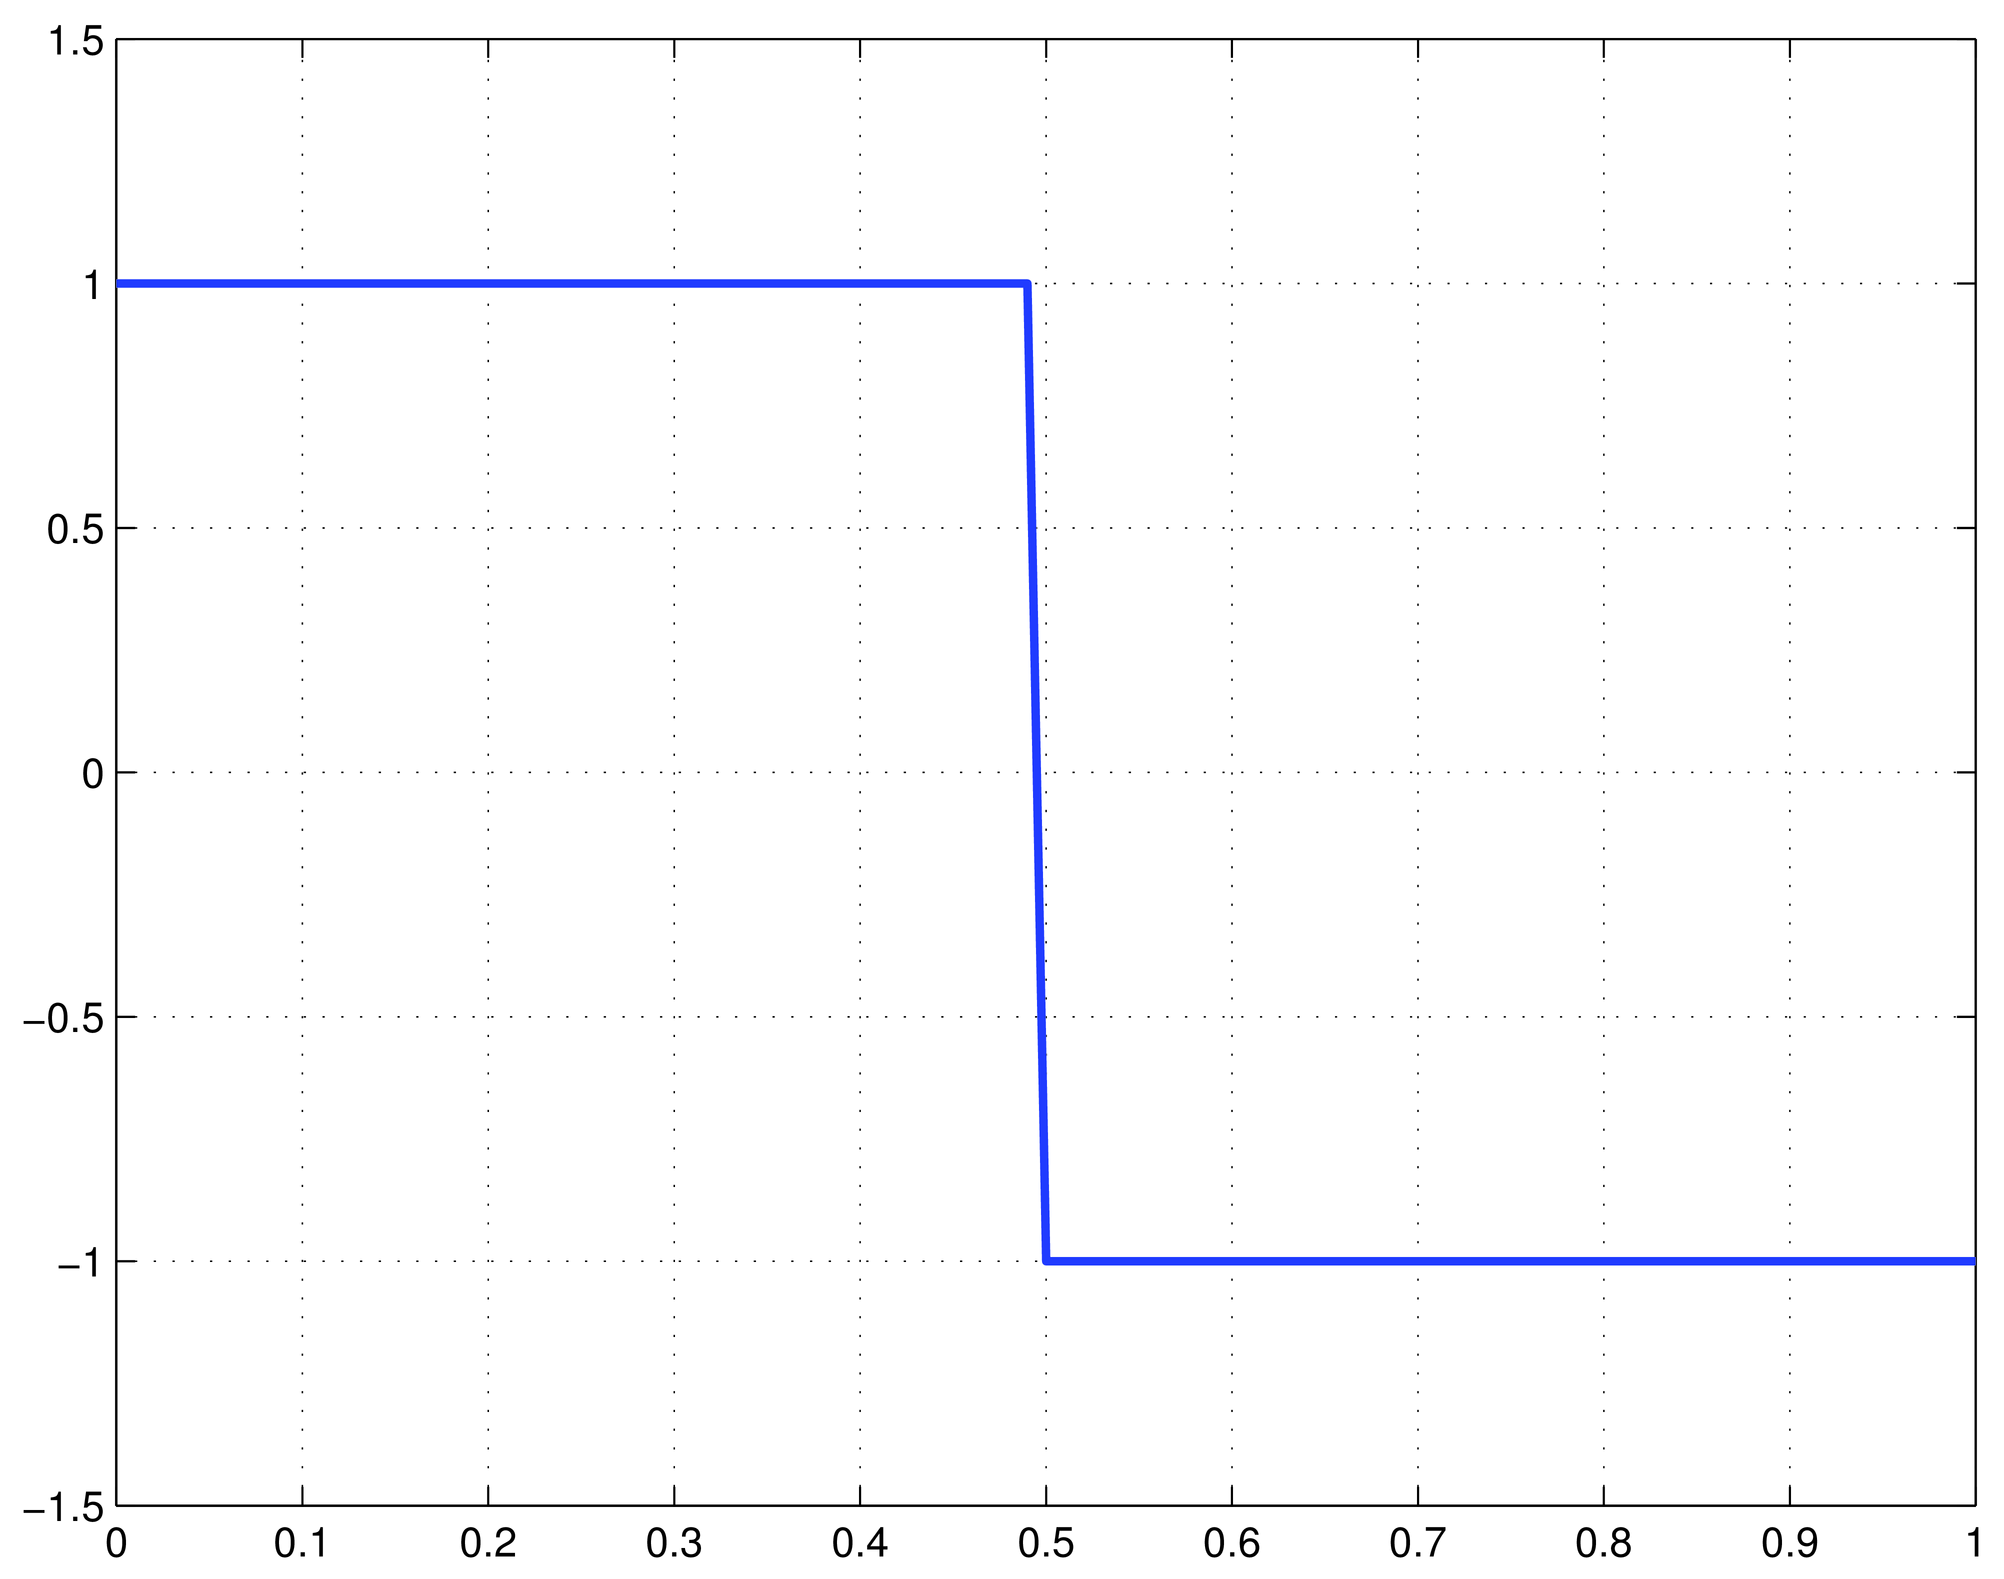
\includegraphics[width=.65\textwidth]{cuadrada}
		\caption{Señal cuadrada de periodo 1 s}
		\label{cuadrada}
		\bigskip
	\end{figure}
\fi

\begin{figure}[h]
\centering
\parbox[t]{0.475\textwidth}{\centering
	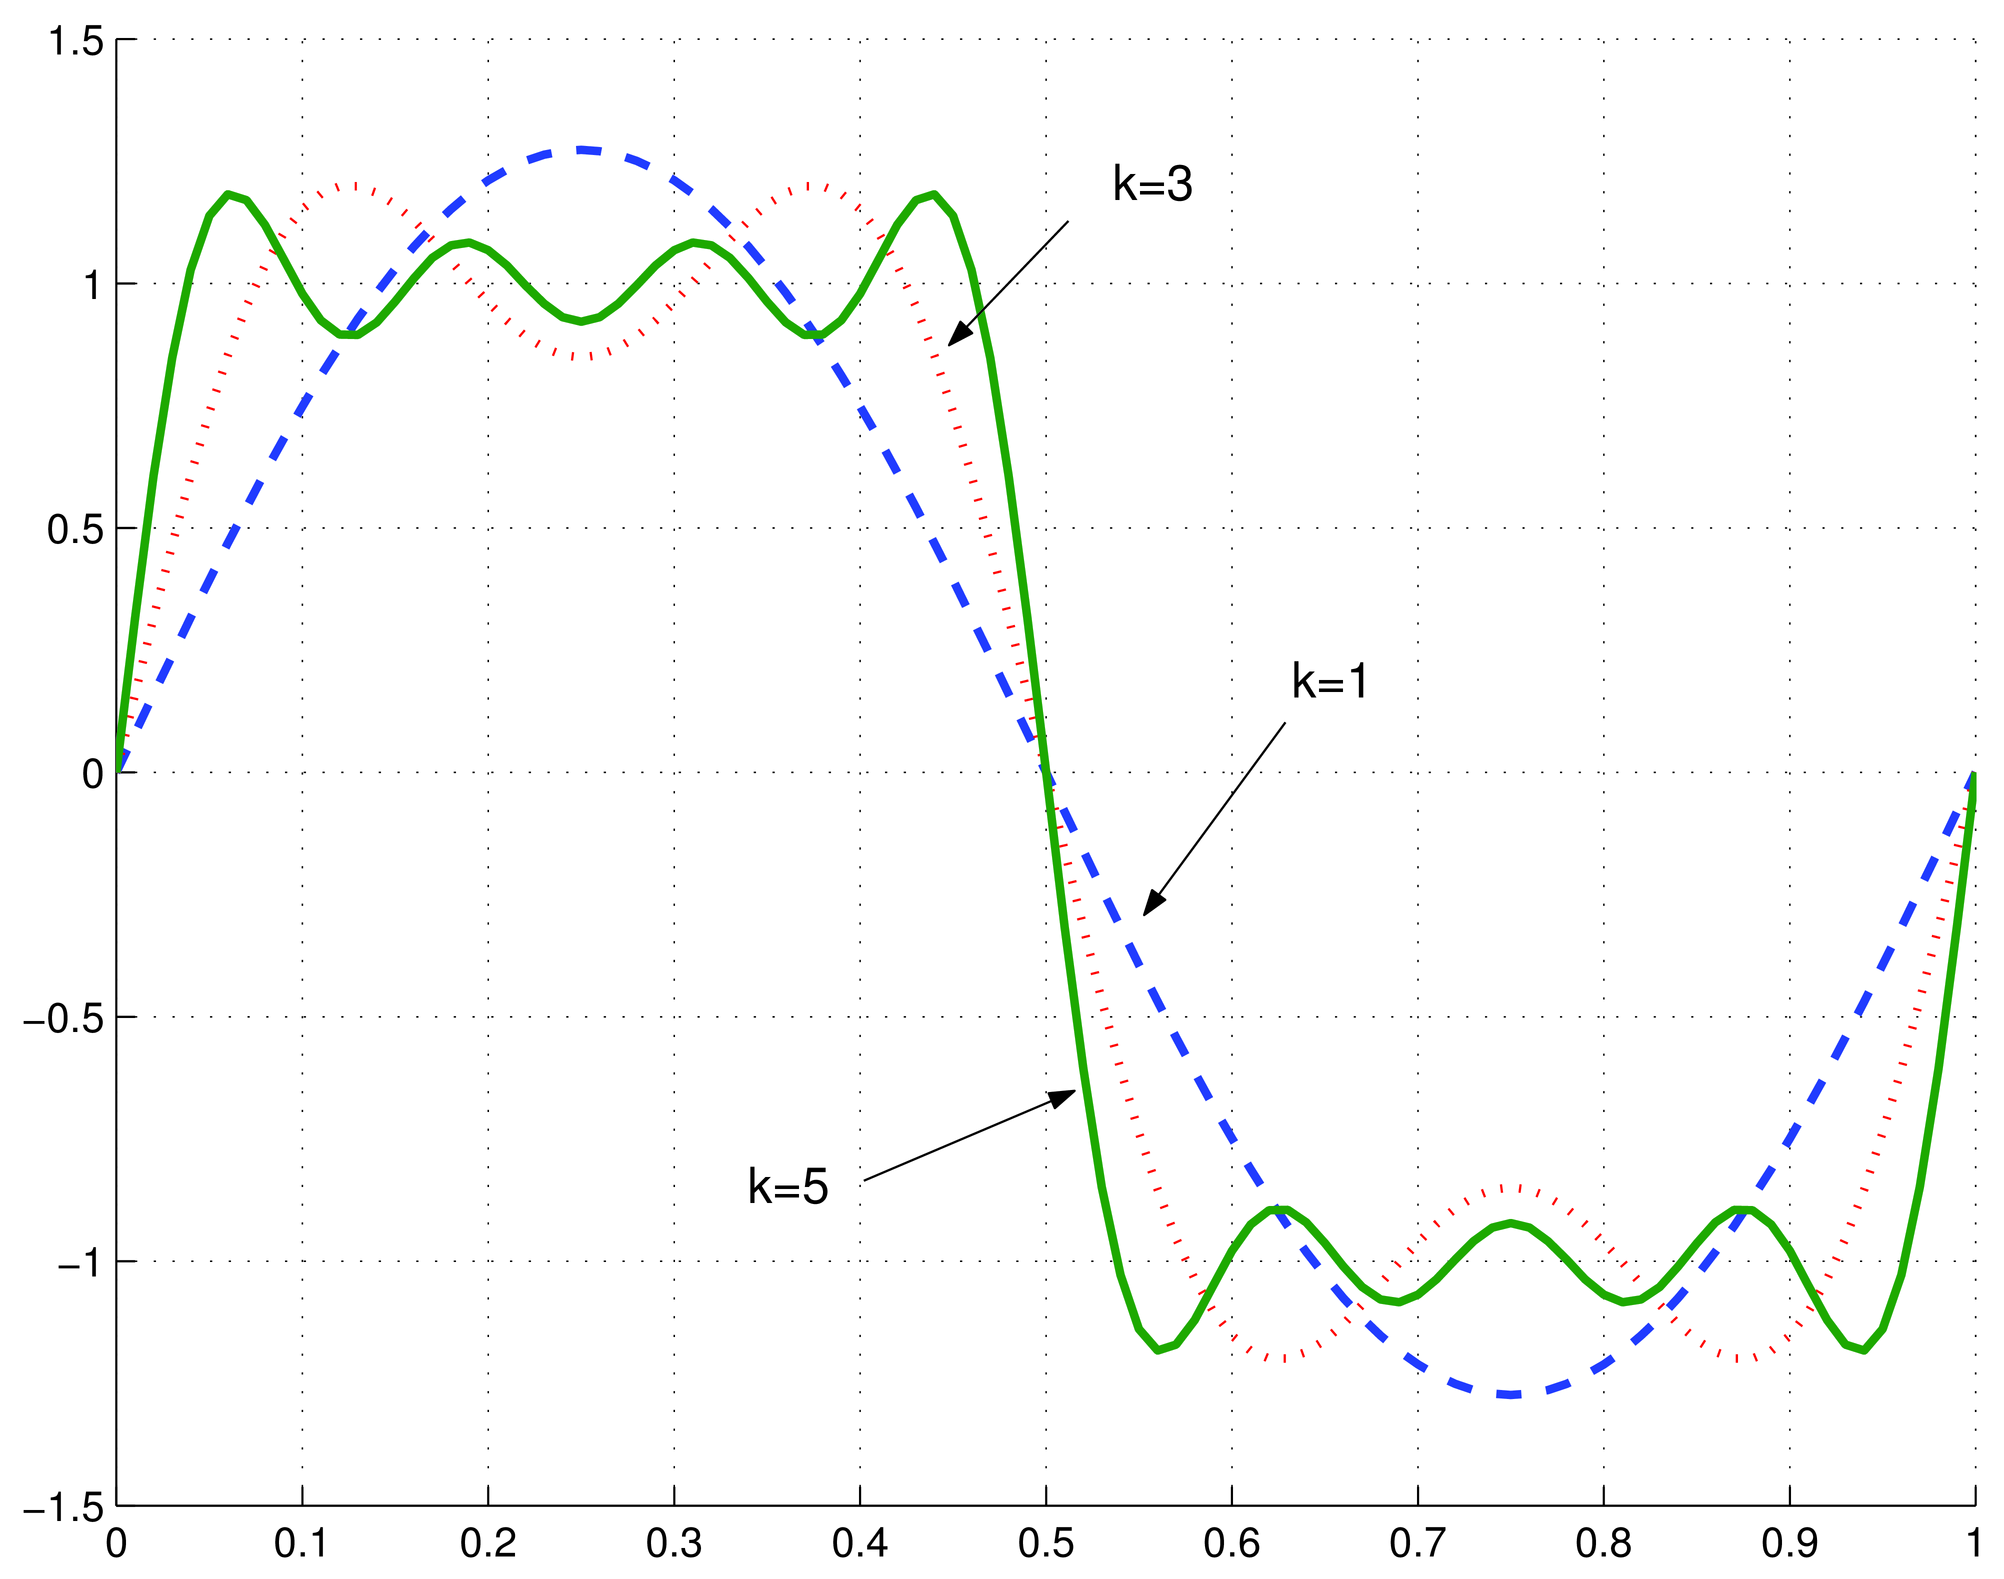
\includegraphics[width = 0.475\textwidth]{fourier}
	\captionof{figure}{Aproximaciones de la señal cuadrada para $k=1,\;2,\;3$}
	\label{fig:fourier}
}
\hfill
\parbox[t]{0.475\textwidth}{\centering
	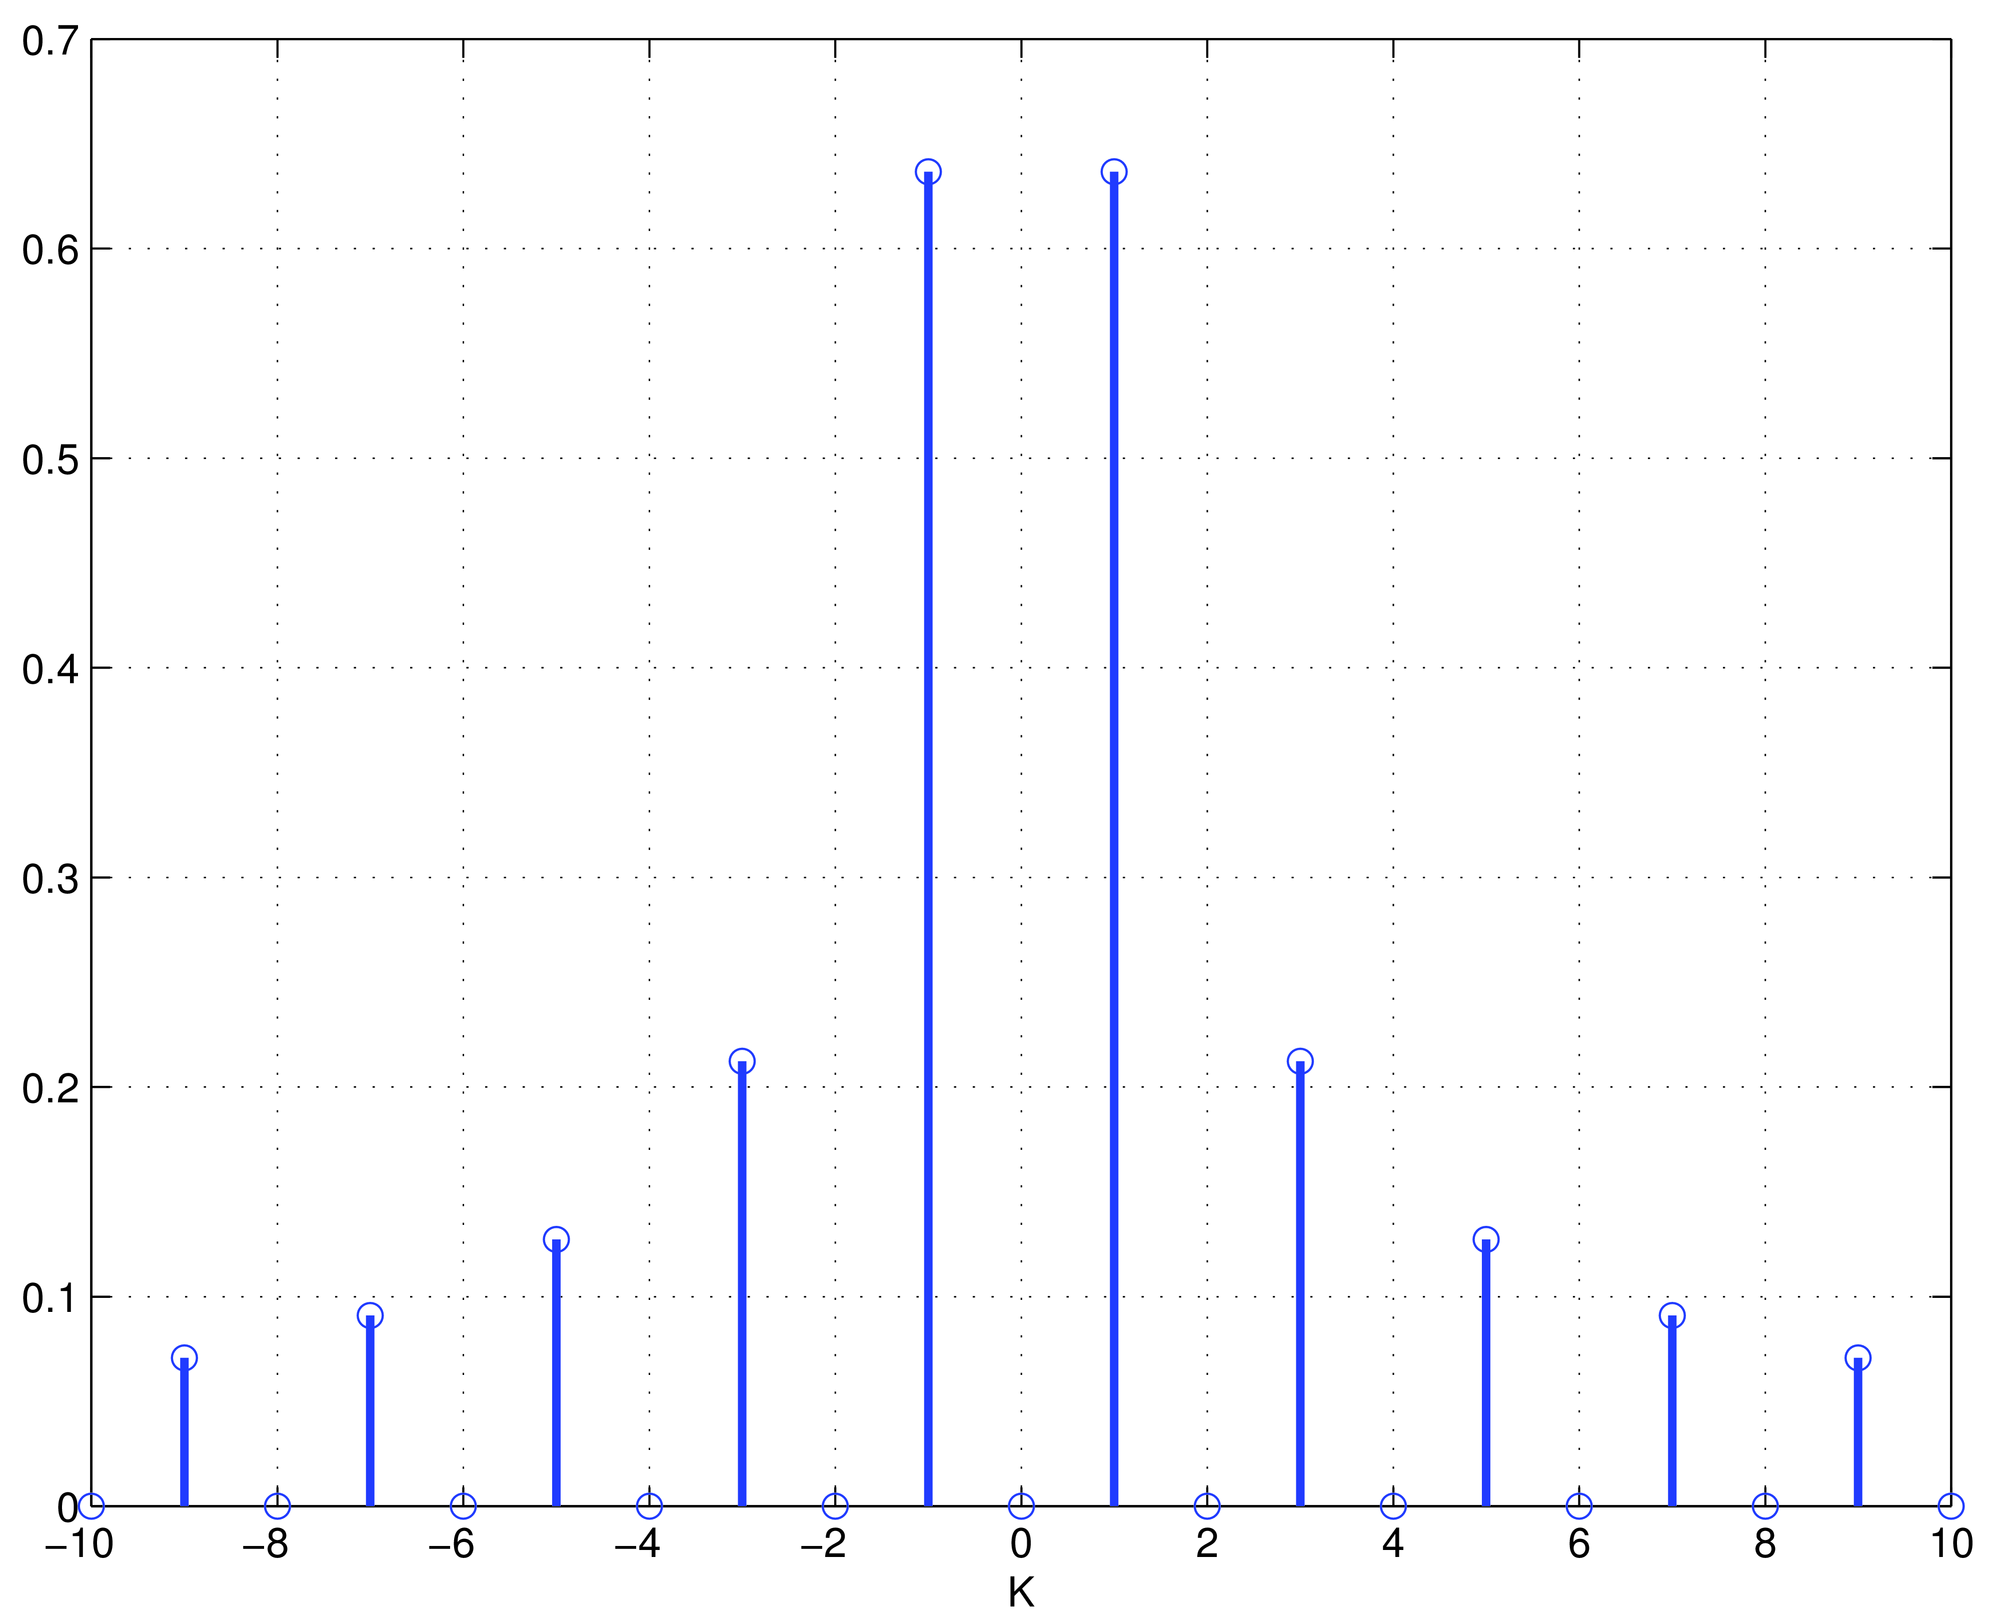
\includegraphics[width = 0.475\textwidth]{espectro}
	\captionof{figure}{Módulo de los factores $g_k$}
	\label{fig:espectro}
}
\end{figure}


El desarrollo en serie Fourier se puede extender al caso de señales aperiódicas mediante la
{\bf Transformada de Fourier}:

\begin{equation*}
	H(j\omega) = \int_{-\infty}^{\infty}g(t)\on{e}^{-j\omega t}dt
\end{equation*}

esta expresión es una generalización de la serie de Fourier \eqref{SerieFourier} que
abarca todas las frecuencias desde cero a infinito (negativas y positivas), además de las que
son múltiplo entero de la frecuencia.

A partir del conocimiento de la transformada de Fourier de una señal es posible obtener ésta
mediante la fórmula de inversión de Fourier:

\begin{equation*}
	g(t) = \dfrac{1}{2\pi}\int _{-\infty}^{\infty} H(j\omega)\on{e}^{j\omega t}d\omega
\end{equation*}

En la \autoref{tabla} se muestran algunas transformadas de Fourier. La interpretación física de la transformada de Fourier de una señal cualquiera es que
proporciona la información sobre el contenido en frecuencia de la misma: \textsl{su espectro en
frecuencia}.

\begin{table}[htb]
	\bigskip
	\begin{center}
		\caption{Tabla con algunas transformadas de Fourier}\label{tabla}
		\begin{tabular}{c c}
			\toprule
			$g(t)$ & $H(j\omega )$ \\[1ex] \midrule 
			$\delta(t)$ & 1 \\[1ex] 
			$\epsilon(t)$ & $\dfrac{1}{j\omega}+\pi\delta(\omega)$ \\[3ex]
			$e^{j\omega_0t}$ & $2\pi\delta(\omega-\omega_0)$ \\[2ex] 
			$\cos(\omega_0t)$ & $\pi\left[\delta(\omega-\omega_0) + 
				\delta(\omega+\omega_0)\right]$ \\[2ex] 
			$\sin(\omega_0t)$ & $\dfrac{\pi}{j}\left[\delta(\omega-\omega_0) - 
				\delta(\omega+\omega_0)\right]$ \\[2ex]
			\bottomrule
		\end{tabular}
	\end{center}
\end{table}


La conclusión más importante de esta primera sección del tema es la siguiente:

\begin{parrafoDestacado}

Cualquier señal, sea periódica o no, se puede descomponer
como una suma o integral (si es aperiódica) de señales armónicas exponenciales con frecuencias entre
$-\infty$ y $\infty$.

\end{parrafoDestacado}

% ----------------------------------------------------------------------------------
\section{Respuesta ante una entrada armónica}
\label{sec:frec:RespArmonicas}

En esta sección se desarrollará la metodología para el cálculo de la respuesta de un sistema
continuo, en régimen permanente, ante una entrada armónica, puesto que, de acuerdo con la sección
anterior, a partir de este resultado se podrá obtener su respuesta ante cualquier entrada periódica,
o no, en régimen permanente.


Supóngase que se desea obtener la respuesta de un sistema continuo ante la entrada armónica
$A\sen (\omega t)$.  Para realizar el cálculo se pueden emplear varias vías:

\goodbreak{\begin{itemize}
	\item La ecuación diferencial de coeficientes constantes del sistema continuo.
	\item La función de transferencia del mismo.
	\item La respuesta impulsional del sistema.
\end{itemize}}

De las anteriores vías se va a emplear la de la función de transferencia. En la asignatura no
se desarrolla el método de convolución para sistemas continuos, de ahí que la respuesta
impulsional no sea útil, y en concordancia con el tema anterior de \textsl{Análisis de
sistemas}, se busca que el alumno se familiarice con el uso de la función de transferencia para
el análisis de sistemas, ya que las ecuaciones diferenciales son empleadas con profusión en la
mayoría de asignaturas de la titulación en las que se analizan sistemas.

Sea $G(s)$ la función de transferencia de un sistema estable o a lo sumo con un polo en cero. La
transformada de Laplace de esta señal armónica es:

\begin{equation*}
	U(s)=\frac{A\omega}{s^{2}+\omega^{2}} 
\end{equation*}

La transformada de Laplace de la señal de salida viene dada por:

\begin{gather*}
	Y(s) = G(s)U(s) = G(s)\frac{A\omega}{s^{2}+\omega^{2}} = 
		Y_{transitorio}(s) + Y_{permanente}(s)\\ 
	Y(s) = Y_{transitorio}(s) + \frac{as+b}{s^{2}+\omega^{2}} 
\end{gather*}

Descomponiendo en fracciones simples: 

\begin{gather*}
	as+b|_{s=j\omega} = \left[ G(s) \frac{A\omega}{s^{2}+\omega^{2}}
		(s^{2}+\omega^{2})\right]_{s=j\omega } = A\omega G(j\omega ) \\[2ex]
	a = A\on{Im}\left[ G(j\omega)\right]; \qquad 
	b = \omega A\on{Re}\left[ G(j\omega) \right] 
\end{gather*}

Tomando sólo la respuesta correspondiente al régimen permanente:

\begin{multline*}
	Y_{permanente}(s) = \frac{A\on{Im} [G(j\omega)]s +
		\omega A \on{Re}[G(j\omega)]}{s^{2}+\omega^{2}} = \\ 
	= A\on{Im}[G(j\omega)] \frac{s}{s^{2}+\omega ^{2}} + 
		A\on{Re}[G(j\omega)] \frac{\omega}{s^{2}+\omega ^{2}}
\end{multline*}

Aplicando la transformada inversa de Laplace:

\begin{multline}\label{RegPerm}
	y_{permanente}(t) =
		A\on{Im}[G(j\omega)] \cos  (\omega t) + A\on{Re}[G(j\omega)] \sen (\omega t) = \\ 
	= A|G(j\omega)| \sen (\omega t +\arg (G(j\omega)))
\end{multline}


De los desarrollos previos, se pueden deducir las siguientes conclusiones:

\begin{parrafoDestacado}
 
Como se puede apreciar la respuesta en régimen
permanente es una señal armónica de la misma frecuencia que la de entrada, con una amplitud
igual al producto de $|G(j\omega)|$ por la amplitud de la armónica de entrada, y con un desfase
con respecto a la entrada igual a $\arg (G(j\omega))$. $G(j\omega)$ se obtiene cambiando $s$
por $j\omega$ en la función de transferencia $G(s)$.

\end{parrafoDestacado}


\begin{parrafoDestacado}

La respuesta de un sistema continuo ante cualquier entrada
periódica se puede obtener mediante una combinación lineal de sus respuestas ante una serie de
señales armónicas de frecuencia múltiplo entero de aquella.

\end{parrafoDestacado}


Como $G(j\omega)$ se obtiene sustituyendo $s$ por $j\omega$ en la función de transferencia, se
la denomina \textbf{función de transferencia de respuesta en frecuencia}, ya que permite
obtener la respuesta en régimen permanente de un sistema continuo ante una entrada armónica de
frecuencia cualquiera. Además, constituye una generalización de la ganancia estática del
sistema, $G(0)$, ya que ésta permite obtener la respuesta cuando la entrada tiene frecuencia
cero, o sea, es una señal escalón, mientras que la función de transferencia de respuesta en
frecuencia es válida para cualquier frecuencia (incluso cero).

Consecuentemente, conocida la función de transferencia de un sistema $G(s)$ es posible conocer
la respuesta frecuencial del mismo.

% -------------------------------------------------
% -------------------------------------------------

\begin{ejemplo}

Dado el sistema con función de transferencia

\begin{equation*}
	G(s)=\dfrac{3(s+1)}{(s+\num{0.1})(s+10)}
\end{equation*}

calcular su respuesta en régimen permanente cuando $u(t)=\sen(2t)$

Su respuesta viene dada por la expresión \eqref{RegPerm}:

\begin{gather*}
	y(t)= |G(j\cdot 2)| \sen(2t +\arg(G(j\cdot 2))) \\ 
	|G(j\cdot 2)|=\dfrac{3|2j+1|}{|2j+\num{0.1}||2j+10|} = \num{0.3285} \\ 
	\arg\left(G(j\cdot 2))= \arg (\dfrac{3(2j+1)}{(2j+\num{0.1})(2j+1)}\right)=\SI{-1.9845}{\radian}
\end{gather*}
	
Luego:

\begin{equation*}
	y(t)=\num{0.3285} \cdot \sen (2t-\num{1.9845})
\end{equation*}

En la \autoref{fig_RegPerm} se muestran la señal de entrada y la correspondiente salida en
régimen permanente. Como se puede apreciar la salida posee una amplitud menor que la entrada y
está desfasada aproximadamente 1 segundo con respecto a ésta.

\end{ejemplo}

% -------------------------------------------------
% -------------------------------------------------

\begin{figure}[h!]\centering
	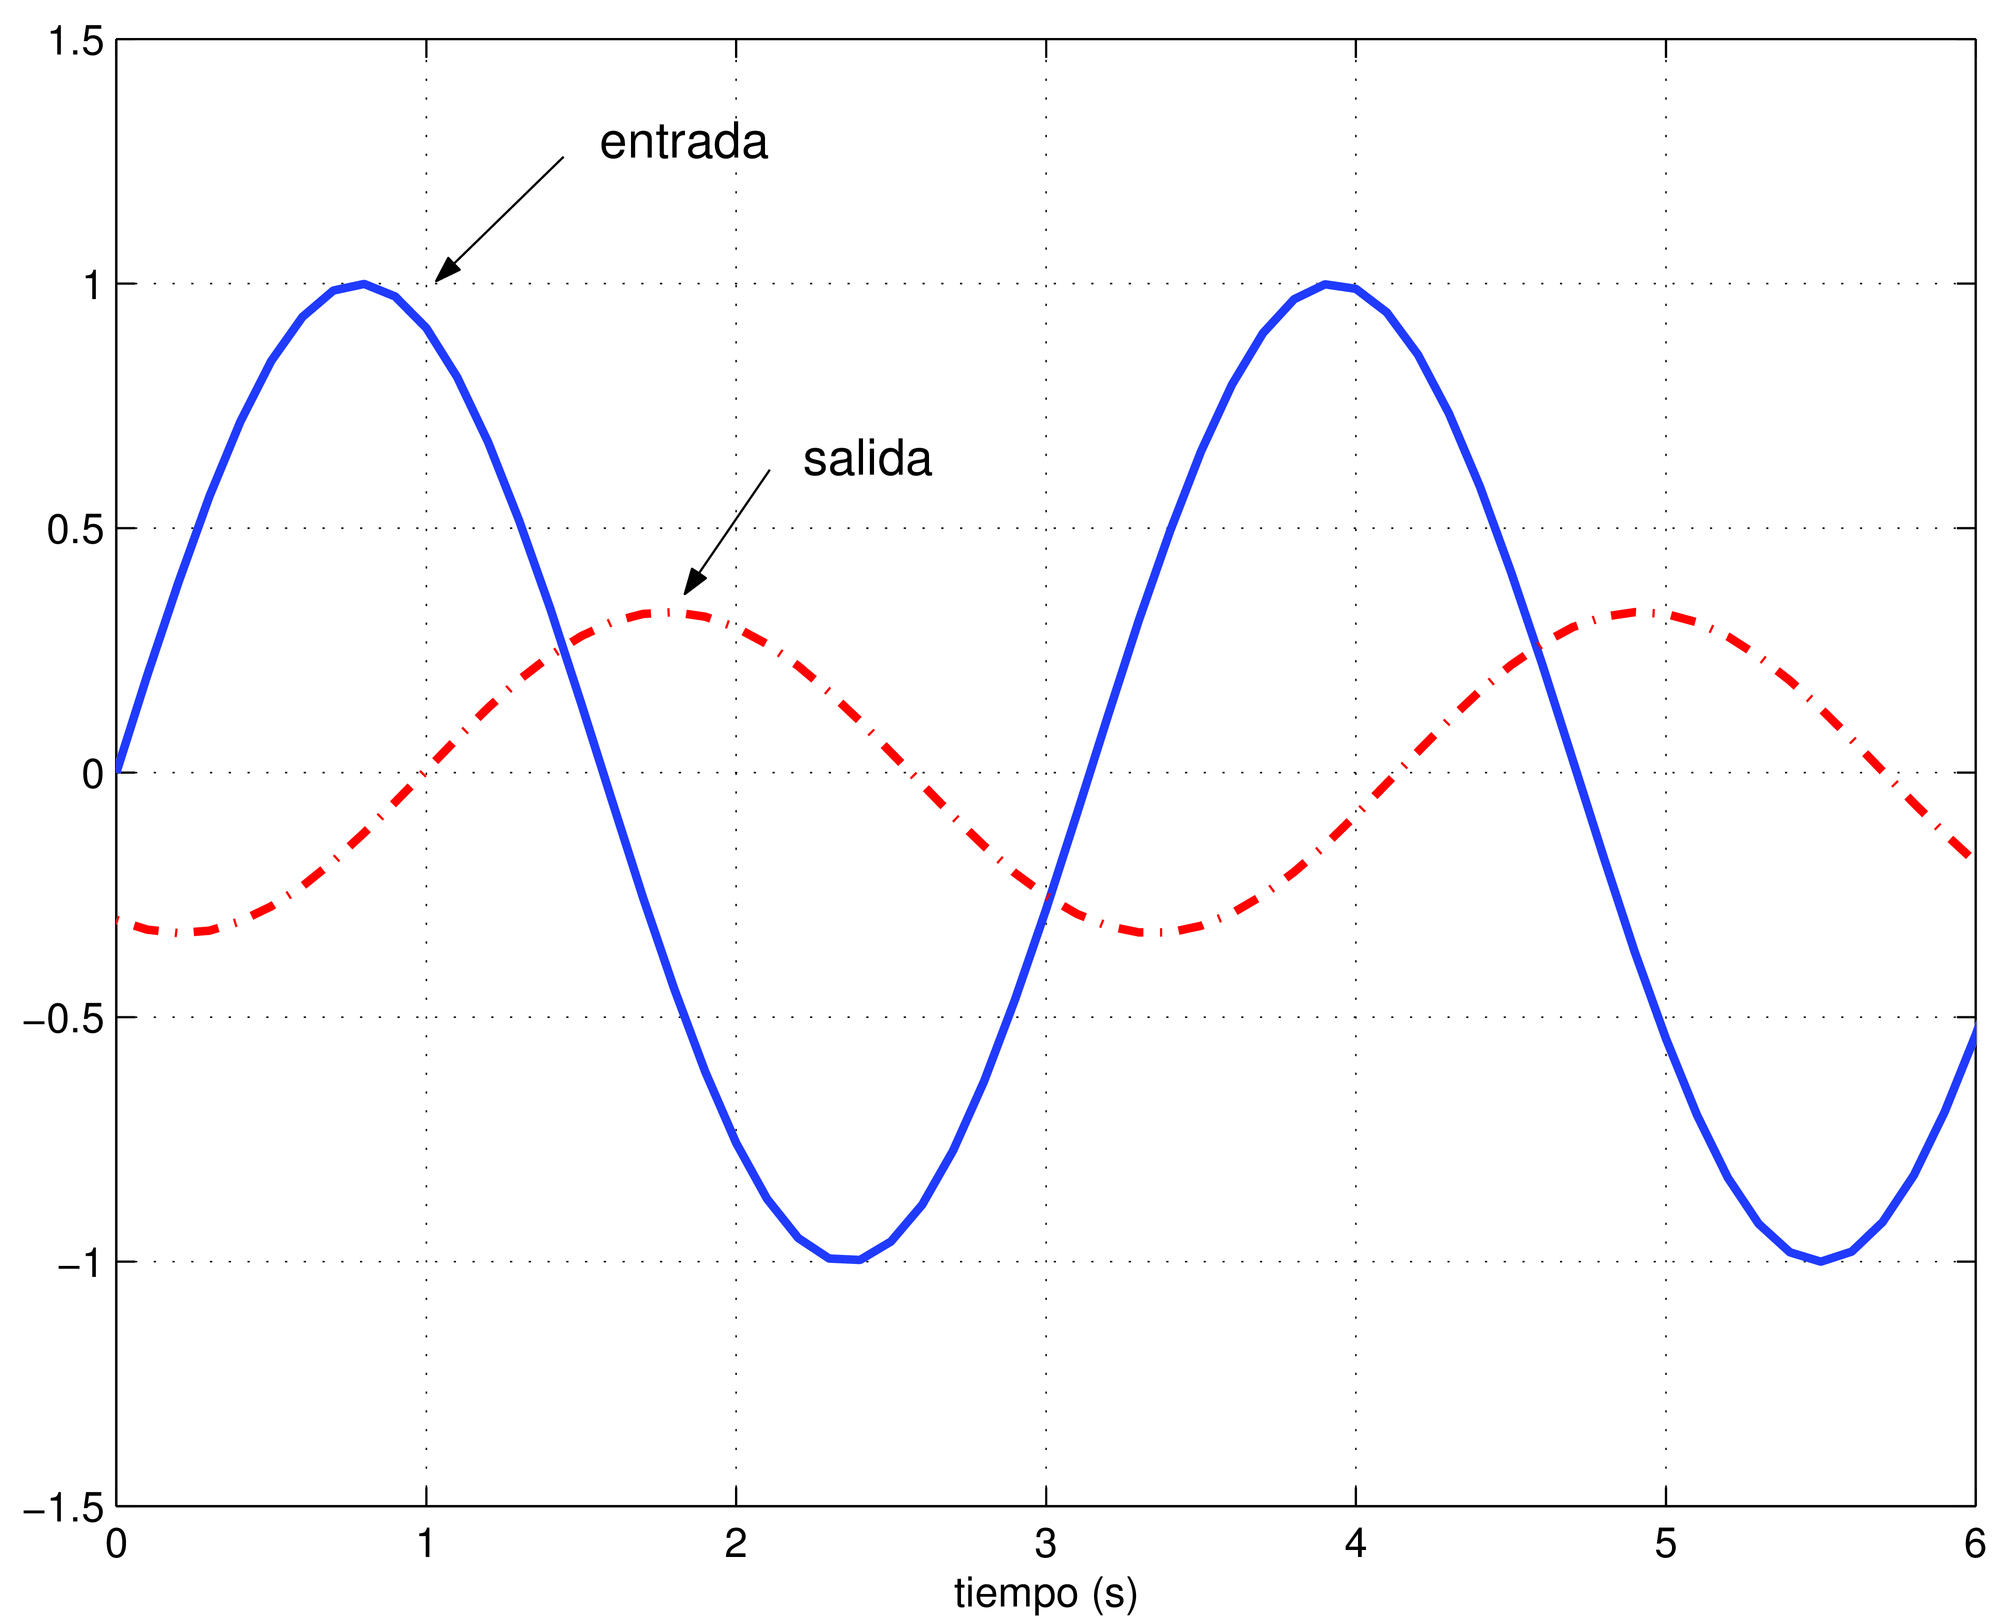
\includegraphics[width=0.65\textwidth]{RegPerm}
	\caption{Representación gráfica de la señal de entrada y de la de salida}\label{fig_RegPerm}
	\bigskip
\end{figure}

Si $|G(j\omega)|>1$ entonces el sistema amplifica la señal de entrada, pues la salida tendrá
una mayor amplitud que ésta, mientras que si $|G(j\omega)|<1$ entonces el sistema atenúa la
señal de entrada. Por ello, al término $|G(j\omega)|$ también se le conoce como ganancia en
frecuencia.
